\section{Methods}

\todo[inline]{put FBA and ll FBA in standard form}
\todo[inline]{how SCIP and HiGHS solve}
\todo[inline]{mention big M value}
\todo[inline]{explain why indicators constraints can be used in CB}

\subsection{test if flux is feasible}
For a given flux distribution $\widetilde{v}$ and the corresponding directions $\widetilde{a}$ the following problem is feasible if it is loopless:
\begin{maxi!}
    {\scriptstyle \Delta \mu, \mu}{0}{\label{Eq:feasiblityCheck}}{} 
    \addConstraint{-M \leq \Delta \mu_i \leq - 1 \quad} {\forall i \in \mathcal{I}: \widetilde{a_i} = 1}    
    \addConstraint{1 \leq \Delta \mu_i \leq M \quad} {\forall i \in \mathcal{I}: \widetilde{a_i} = 0}        
    \addConstraint{\Delta \mu \tran = \mu \tran S_{int}}{}
    % \addConstraint{\mu \in \mathbb{R}^m}
    % \addConstraint{\Delta \mu \in \mathbb{R}^n}
    % \addConstraint{v \in \mathbb{R}^n}
    % \addConstraint{S \in \mathbb{R}^{m\times n}}
\end{maxi!} 
Note that if $\widetilde{v_i} = 0$, the reaction can be removed from the problem by removing the reaction from $S_{int}$ and without adding variable $\Delta \mu_i$. 

Problem \cref{Eq:feasiblityCheck} can also be used to test the looplessness of a solution and a subset of internal reactions by setting the flux of all other reactions to zero.

\subsection{block cycles in FBA solution}

\subsection{No good cuts}
The following "relaxed" version of \cref{Eq:thermoFba} is solved, where the thermodynamic feasibility is ignored, but the indicator variables $a$ are kept:
\begin{maxi!}
    {\scriptstyle v, a}{c\tran v}{\label{Eq:noGoodCut}}{} 
    \addConstraint{Sv=0} 
    \addConstraint{l \leq v \leq u}
    \addConstraint{a_i = 1}{\quad \implies \quad v_i \geq 0}{\quad \forall i \in \mathcal{I}}      \addConstraint{a_i = 0}{\quad \implies \quad v_i \leq 0}{\quad \forall i \in \mathcal{I}}
\end{maxi!}

If a solution to \cref{Eq:noGoodCut} is thermodynamically infeasible, the following constraint is added to \cref{Eq:thermoFba}:

\begin{equation} \label{noGoodCut}
\sum_{i \in \mathcal{O}} a_i + \sum_{i \in \mathcal{Z}} (1-a_i) \leq |\mathcal{I}|-1
\end{equation}

where $\mathcal{O}$ is the set of $a_i$'s that are assigned to one in the solution and $\mathcal{Z}$ is the set of $a_i$'s that are assigned to zero. The problem is now solved again and this procedure is repeated until the solution is thermodynamically feasible.

\subsection{Combinatorial Benders}
\todo[inline]{move fundamental parts to optimization chapter}
The following ILP is called the master problem (MP) of \cref{Eq:deltaM}: \todo{fix reference}
\begin{maxi!}
    {\scriptstyle v, a}{c \tran v}{\label{Eq:masterProblem}}{} 
    \addConstraint{Sv=0} 
    \addConstraint{l \leq v \leq u}
    \addConstraint{a_i = 1}{\quad \implies \quad v_i > 0}{\quad \forall i \in \mathcal{I}}      \addConstraint{a_i = 0}{\quad \implies \quad v_i < 0}{\quad \forall i \in \mathcal{I}}
\end{maxi!}

 The sub problem (SP) is the \textit{parameterised program}:
\begin{maxi!}
    {\scriptstyle \mu}{0}{\label{Eq:subProblem}}{} 
    \addConstraint{\widetilde{a_i} = 1}{\quad \implies \quad (S_{int} \tran \mu)_i < 0}{\quad \forall i \in \mathcal{C}}
    \addConstraint{\widetilde a_i = 0}{\quad \implies \quad (S_{int} \tran \mu)_i > 0}{\quad \forall i \in \mathcal{C}}
    % \addConstraint{c \tran v \geq \mathcal{UB} + \epsilon}
\end{maxi!}

where $\widetilde{a}$ is fixed to the values of a solution to the master problem and $\mathcal{C}$ a corresponding minimal infeasible subsystem (MIS). The following Combinatorial Benders' (CB) cut is added to the master problem if the sub problem is infeasible:

\begin{equation*}
\sum_{i \in \mathcal{C}: \widetilde{a_i}=0} a_i + \sum_{i \in \mathcal{C}: \widetilde{a_i}=1} (1-a_i) \geq 1
\end{equation*}

This process is repeated until a solution is found, that is feasible in the master problem and the sub problem and therefore also for \cref{Eq:deltaM}.

Note that if $\mathcal{C}$ contains all internal reactions $\mathcal{I}$, the CB cut is a no good cut \cref{noGoodCut}.


\subsubsection*{minimal infeasible subset}
\todo[inline]{rephrase section}
If a solution to the master problem \cref{Eq:masterProblem} is not loopless, the following primal linear program \cref{Eq:subProblem} is infeasible:
% To find minimal infeasible subsets, the following primal linear program of an infeasible solution \cref{Eq:subProblem} is formulated: 
\begin{maxi!}
    {\scriptstyle \mu}{0}{\label{Eq:MISPrimal}}{} 
    \addConstraint{\widetilde{a_i} = 1}{\quad \implies \quad (S_{int} \tran \mu)_i < 0}{\quad \forall i \in \mathcal{I}}
    \addConstraint{\widetilde a_i = 0}{\quad \implies \quad (S_{int} \tran \mu)_i > 0}{\quad \forall i \in \mathcal{I}}
\end{maxi!}

We use the infeasible primal problem \cref{Eq:MISPrimal} and its corresponding dual problem \cref{Eq:MISDual} to generate a minimal feasible set. 

First, the primal problem is transformed in standard form \todo{standard form defined earlier requires $x \geq 0$}.
To construct the matrix of inequalities $\widetilde{A}$, the inequalities are brought in standard form. Slack variables are added to have inequalities instead of strict inequalities: 
\begin{equation*}
    (S_{int} \tran \mu)_i < 0 \implies (S_{int} \tran \mu)_i + \epsilon \leq 0 \implies (S_{int} \tran \mu)_i \leq - \epsilon \\
\end{equation*}
\begin{equation*}
    (S_{int} \tran \mu)_i > 0 \implies (S_{int} \tran \mu)_i - \epsilon \geq 0  \implies (S_{int} \tran \mu)_i \geq \epsilon
\end{equation*}

To have the decision variable $\mu$ on the left hand side of $\geq$, the constraint is multiplied by -1:
\begin{equation*}
    (S_{int} \tran \mu)_i \leq - \epsilon \implies - (S_{int} \tran \mu)_i \geq \epsilon
\end{equation*}

The primal in standard form is then:
\begin{maxi!}
    {\scriptstyle \mu}{0}{\label{Eq:MISPrimalStandard}}{} 
    \addConstraint{\widetilde{A} \mu \geq \widetilde{b}}
\end{maxi!}
where $\widetilde{b} = \epsilon^{\dim(\mathcal{I})}$ and row $i$ of $\widetilde{A}$ is the row of $-(S_{int} \tran)$ if $\widetilde{a_i} = 1$ and of $(S_{int} \tran)$ if $\widetilde{a_i} = 0$. 

% The Lagrangian of \cref{Eq:MISPrimal} is thus: 
% \begin{equation*}
%     \mathcal{L} (\mu, \lambda) = 0 + \lambda \tran (\widetilde{A} \mu - \widetilde{b})
% \end{equation*}
% where $\lambda \geq 0$ the Lagrange multiplier for the inequality constraints. 

% \begin{align*}
%     \max_{\mu} \quad \mathcal{L}(\mu, \lambda) & = \max \quad \lambda \tran (\widetilde{A} \mu - \widetilde{b}) &\\
%     & = \max \quad \lambda \tran \widetilde{A} \mu - \lambda \tran \widetilde{b} &\\
%     & = \max \quad \mu \tran (\widetilde{A} \tran \lambda) - \widetilde{b} \tran \lambda &\\
%     & = \{
%     \begin{array}{lr}
%         - \widetilde{b} \tran \lambda &\text{if} \quad \widetilde{A} \tran \lambda = 0,\\
%         \infty &\text{otherwise}
%     \end{array}
% \end{align*}

% \cite{boyd_stephen_convex_2004} \cite{aps_mosek_nodate} \cite{bishop_pattern_2006}

The dual problem corresponding to \cref{Eq:MISPrimalStandard} is then: 
\begin{mini!}
    {\scriptstyle \lambda}{- \widetilde{b} \tran \lambda}{\label{Eq:ISDual}}{} 
    \addConstraint{\widetilde{A} \tran \lambda = 0}{}{}
    \addConstraint{\lambda \geq 0}
\end{mini!}

If the primal \cref{Eq:MISPrimalStandard} is infeasible, the dual \cref{Eq:ISDual} is unbounded. As $\lambda$ can be zero, a feasible solution to the dual problem is guaranteed to exist. The scaling of a solution due to unboundedness is not of interest, so any solution can be added as constraint to the dual problem, e.g. $-\widetilde{b} \tran \lambda = -1$. A solution $\lambda^*$ to the dual proves the infeasibility of the primal:
\begin{align*}
    \widetilde{A} \mu \geq \widetilde{b} &\\
    \lambda \tran \widetilde{A} \mu \geq \lambda \tran \widetilde{b} &\\
    0 \geq \lambda \tran \widetilde{b} \quad &(\lambda \tran \widetilde{b} = 1)
\end{align*}

Each vertex of the dual polyhedron has a support defining a minimal infeasible subset. \todo{read paper of Gleeson and Ryan}
To have as few constraints active as possible, it is sufficient to minimize the sum of dual variables: 
\begin{mini!}
    {\scriptstyle \lambda}{1 \tran \lambda}{\label{Eq:MISDual}}{} 
    \addConstraint{\widetilde{A} \tran \lambda = 0}{}{}
    \addConstraint{\widetilde{b} \tran \lambda = 1}{}{}
    \addConstraint{\lambda \geq 0}
\end{mini!}

The non-zero elements in $\lambda$ correspond to a MIS with the set of reaction indices $C$. 

% \unsure[inline]{should we not minimise over the number of non zero lambdas?}
% \unsure[inline]{Is constraint of b even needed??}

\unsure[inline]{What do MIS mean? reactions in cycle?}

By modifying the objective function in \ref{Eq:MISDual} one obtains several minimal infeasible subsets. As proposed in \cite{codato_combinatorial_2006}, coefficients in the objective function can be iteratively set to zero.

\subsection{Intersection Cuts}
\todo[inline]{reference optimization section more}
\todo[inline]{use $\delta$ instead of -1, 1}
In order to apply intersection cuts to the loopless FBA problem \cref{Eq:llfba}, the problem has to be brought in the required form:
\begin{maxi*}
    {\scriptstyle x}{c \tran x}{\label{Eq:mathematical_program_S_P_2}}{} 
    \addConstraint{x \in S \cap P}
\end{maxi*}
We set $x = (v, \Delta \mu, \mu)$, where $v \in \mathbb{R}^n$, $\Delta \mu \in \mathbb{R}^{\dim (\mathcal{I})}$ and $\mu \in \mathbb{R}^m$. The vector $c \in \mathbb{R}^n$ has the same coefficients as the objective function in FBA \cref{Eq:fba} and a coefficient of $0$ for the variables $\Delta \mu, \mu$. The polyhedral set $P$ contains solutions that respect the steady-state constraints, the bound constraints on $v$ and the constraint \cref{Eq:llfba}(e):
\begin{equation*}
    \centering
    P = \{(v, \Delta \mu, \mu) \, | \, Sv=0, \, l \leq v \leq u, \, \Delta \mu \tran = \mu \tran S_{int}\}
\end{equation*}

\cref{Eq:llfba}(d) is captured in the set $S$ by using the same approximation as in \cref{Eq:thermo_fba_indicator} and \cref{Eq:thermo_fba_bigM}:
for any internal reaction $i$ the flux through the reaction $v_i$ and $\Delta \mu_i$ are of opposite sign unless $v_i=0$ in which case $\Delta \mu_i$ can be positive or negative but cannot be in the interval $(- \delta, \delta)$. $S$ is closed as it is defined using inclusive inequalities and therefore it contains its limit points. 
\begin{align*}
    \centering
    %S &= \{(v_i, \Delta\mu_i) \, | \, \Delta \mu_i v_i < 0 \lor v_i = 0 \quad \forall i \in \mathcal{I}\} \\
    S &= \{(v_i, \Delta\mu_i) \, | \, (v_i \geq 0, \, \Delta \mu_i \leq - \delta) \lor (v_i \leq 0, \, \Delta \mu_i \geq \delta) \quad \forall i \in \mathcal{I}\}
\end{align*}
The intersection of $P$ and $S$ is the feasible region of the ll-FBA problem. 
\todo[inline]{define A, b (to understand what $\tilde A$) means later}

As explained in \cref{intersection_cuts}, in order to get an intersection cut we require an $S$-free set $C$ containing the relaxed solution $\tilde x$. Let $\tilde x = (\tilde v, \tilde {\Delta \mu}, \tilde \mu)$ be an optimal solution to the relaxed LP which is in $P$ but not in $S$. There must be at least one reaction $i$ for which holds $\Delta \mu_i v_i > 0$ \todo{include interval -1, 1}. One of the maximal $S$-free sets below contains such an optimal solution:
\begin{align*}
    C_1 &= \{(v_i, \Delta\mu_i) \, | \, \Delta \mu_i \geq -1, \, v_i \geq 0\} \\
    C_2 &= \{(v_i, \Delta\mu_i) \, | \, \Delta \mu_i \leq 1, \, v_i \leq 0\} %\\
    % C_3 &= \{(v_i, \Delta\mu_i) \, | \, -1 \leq \Delta \mu_i \leq 1 \, v_i \in \mathcal{I} \}
\end{align*}
\unsure[inline]{add two more plots for other S-free sets}
\todo[inline]{add $C_3$? can be tilted}
Suppose that $\tilde v_i > 0$ and $\tilde{\Delta \mu_i} > -1$. Such a solution is not in $S$ but contained in $C_1$ \todo{projected into space of $(v_i \Delta \mu_i)$}. A diagram for this case is shown in \cref{fig:intersection_cut}. If $\tilde v_i < 0$ and $\tilde{\Delta \mu_i} < 1$ the solution is contained in $C_2$.

\begin{figure}[h!]
    \caption{diagram of an intersection cut for ll-FBA}
    \centering
    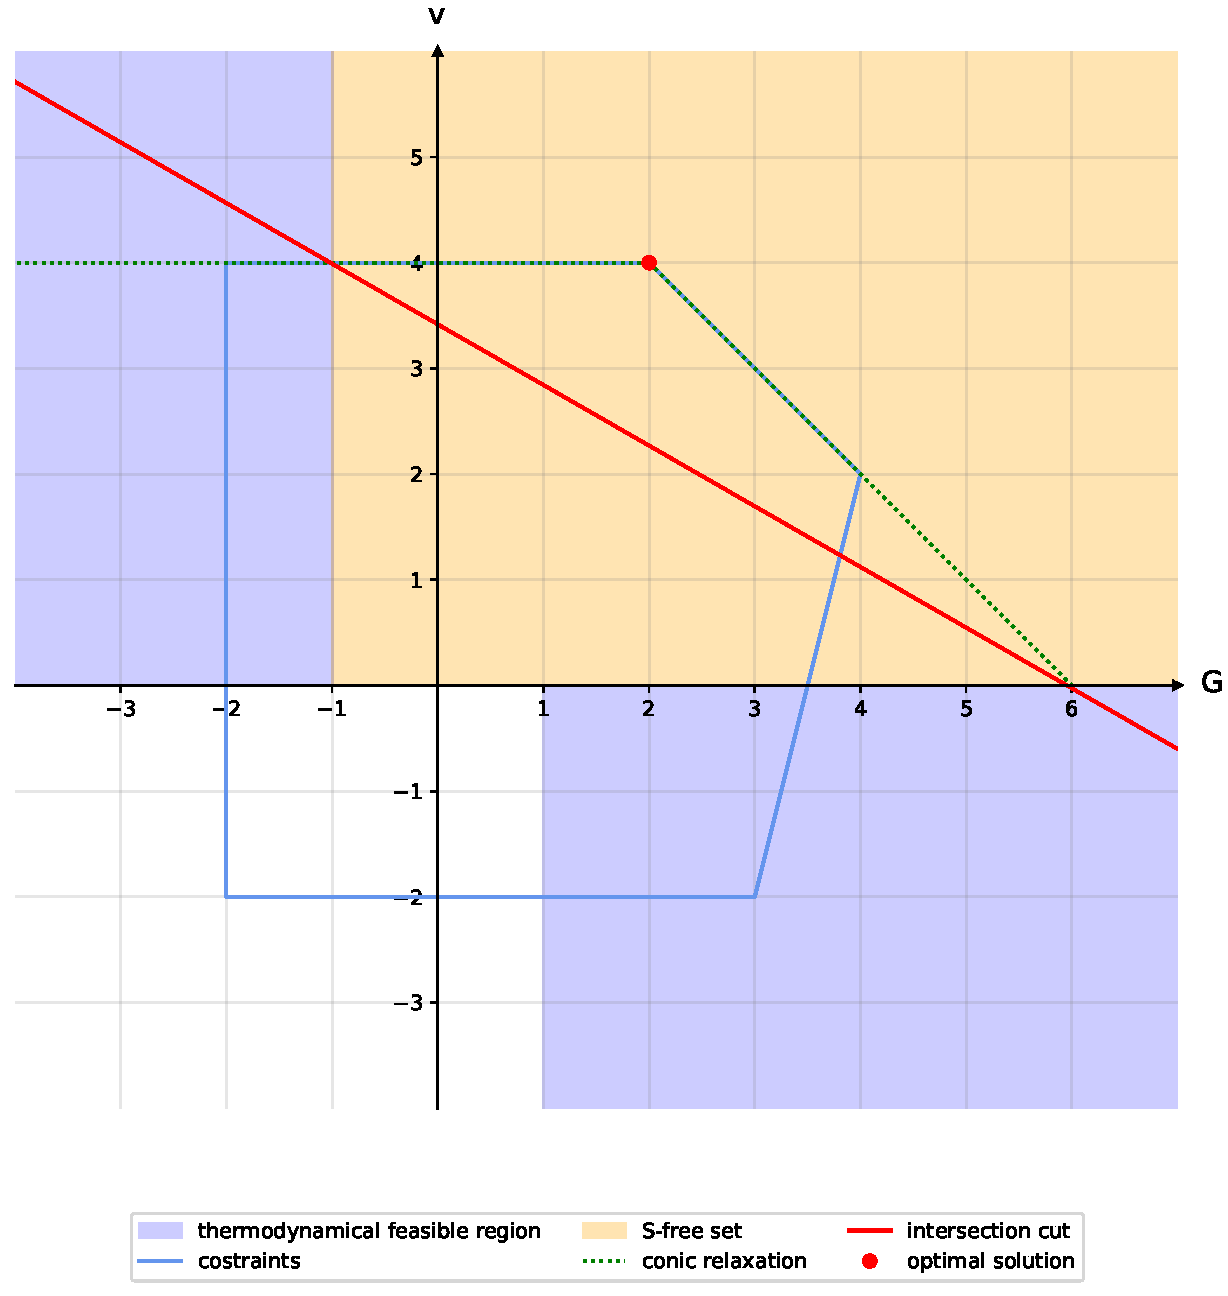
\includegraphics[width=0.8\textwidth]{Images/intersection_cut_ll_fba.pdf}
    \label{fig:intersection_cut_ll_fba}
    \subcaption{A simplified problem in 2D: we have the decision variables $v, \Delta \mu \in \mathbb{R}$. We have polyhedral constraints $P$ (blue) and the set $S$ (purple area). The intersection of $S$ and $P$ is the true feasible region. Let the optimal solution to the relaxed problem be at $(2,4)$. As $v$ and $\Delta \mu$ in the optimal solution to the relaxed ll-FBA are both positive $C_1$ is a maximal $S$-free set (yellow area). The conic relaxation at $\tilde x$ and the S-free set $C_1$ intersect at the points $(-1,4)$ and $(6,0)$. The area between the line through the intersecting points and $\tilde x$ is cut off.}
\end{figure}

\todo[inline]{make figure nice, correct labels, colour interior of polytope, do not call it 2D, fix cut off extreme ray}

The conic relaxation $P'$ at a relaxed solution $\tilde x$ is a cone with apex $\tilde x$ the extreme rays are the intersections of the active constraints. $P'$ can be written as a conic combination of extreme rays \cref{Eq:conic_relaxation} or as a polyhedron of the active constraints \cref{Eq:conic_relaxation_polyhedral}. The basic variables and nonbasic constraints defining a basis $P'$ for $\tilde x$ can be extracted from an LP solver. 

Suppose reaction $i$ in $\tilde x$ has $\tilde v_i >0$ and $\tilde{\Delta \mu_i} >-1$. $(\tilde v_i, \tilde{\Delta \mu_i}) \in C_1$ and $(\tilde v_i, \tilde{\Delta \mu_i}) \not \in C_2$ and therefore $C_1$ is a maximal $S$-free set around $\tilde x$.
To compute the intersection of the conic relaxation and $C_1$, we check for each extreme ray $r^j = (- \tilde A^{-1}_{*,j})$ generated by $\tilde x$ whether it intersects the boundary of $C_1$. 
First, the intersection of the conic relaxation with the hyperplane $h_1 = \{ x \in \mathbb{R}^{n + m + |\mathcal{I}|} \, | \, v_i = 0 \} $ is computed. $(\tilde x + \lambda_1 r^j)_{k_1} = 0$ is solved for $\lambda_1$, where $k_1$ corresponds to the index of $v_i$ in $\tilde x$.
% Each ray $r^j$ generated by $\tilde x$ is set equal to $h_1$ and solved for $\lambda_1$: $\tilde x + \lambda_1 r^j=h_1$. 

Similarly, the intersection of each extreme ray generated by $\tilde x$ with $h_2$ is computed, where $h_2 = \{ x \in \mathbb{R}^{n + m + |\mathcal{I}|} \, | \, \Delta \mu_i = -1 \}$. We solve $(\tilde x + \lambda_2 r^j)_{k_2} = -1$ for the step size $\lambda_2$, where $k_2$ is the index of $\Delta \mu_i$ in $\tilde x$. 
An extreme ray intersects the boundary of $C_1$ if either $\lambda_1$ or $\lambda_2$ is finite and positive. If $\lambda_1, \lambda_2$ are both negative or if the ray does not intersect with either of the lines, there is no intersection with $C_1$ and the step size is set to $\infty$. 
\todo[inline]{explain what happens if lambda is zero or very small, or if lines are almost parallel \\ explain the geometric meaning of infinity case}

If reaction $i$ in $\tilde x$ has $v_i <0$ and $\Delta \mu_i <1$, the intersection between the conic relaxation and $C_2$ is computed analogously. The equations to solve are $(\tilde x + \lambda_1 r^j)_{k_1} = 0$ and $(\tilde x + \lambda_1 r^j)_{k_2} = 1$.

% Suppose we have one reaction and $v, \Delta \mu \in \mathbb{R}$ which have positive values assigned. The $S$-free set $C_1$ contains the points that are greater than $s_1 = \begin{pmatrix} 1 \\ 0 \end{pmatrix} t_1$ and greater than $s_2 = \begin{pmatrix} -1 \\ 0
% \end{pmatrix} + \begin{pmatrix} 0 \\ 1 \end{pmatrix} t_2$ \todo{make vector nice}. First, the intersection of the conic relaxation with the line $s_1$ is computed. Each ray $r^j$ generated by $\tilde x$ is set equal to $s_1$ and solved for $\lambda_1$: $\tilde + \lambda_1 r^j=s_1$. Analogously, each ray generated by $\tilde x$ is set equal to $s_2$ and the step size is denoted as $\lambda_2$. The intersection with the boundary of $C_1$ is the minimum of positive $\lambda_1$ and $\lambda_2$. If $\lambda_1, \lambda_2$ are both negative or if the ray does not intersect with either of the lines, there is no intersection with $C_1$ and the step size is set to $- \infty$.
% In higher dimensions, the $S$-free set  of reaction $i$ with $v_i > 0$ and $\Delta \mu_i > -1$ is still the intersection of the two half-spaces $C_1 = \{(v, \Delta \mu) | v_i \geq 0, \, \Delta \mu_i \geq -1\}$.

% There are at least two possibilities of using intersection cuts: (1) one can either decompose the problem to solve FBA ... \todo{depends on definition of $P$} and generate cuts based on a solution to the master problem or 
% (2) one could also compute several intersection cuts from an FBA solution and add the cuts to the ll-FBA problem. 

\todo[inline]{write about possible usage of intersection cut}

